% Generated from THESIS_DRAFT.md.
\chapter{Bộ nhớ sự kiện thị giác cho SmolVLA}

\section{Tiến độ tác vụ và giả thuyết biểu diễn}

Tác vụ T1 và T3 yêu cầu robot nhấc bát và đặt lại trên đĩa ban đầu lần lượt một và ba lần. Gọi $N\in\{1,3\}$ là số chu kỳ được yêu cầu và $z_t$ là số chu kỳ đã thực sự hoàn tất đến bước $t$ theo định nghĩa tác vụ. Một cấu hình nhìn thấy bát ở trên đĩa có thể xuất hiện ở nhiều giá trị $z_t$. Trong trường hợp hai lịch sử dẫn đến cùng quan sát tại lúc bát nằm trên đĩa, một chính sách chỉ điều kiện hóa trên quan sát đó và cùng chỉ dẫn sẽ sinh cùng phân phối hành động. Tuy nhiên, vai trò của một chu kỳ tiếp theo thay đổi theo tiến độ. Khi $z_t<N$, chu kỳ tiếp theo có thể đưa tác vụ đến đích. Khi $z_t=N$, một chu kỳ mới có thể gây vượt mục tiêu. Ví dụ này giải thích vì sao số chu kỳ là một biến lịch sử có ý nghĩa cho thiết kế. Tần suất các quan sát tương đương trong các lượt chạy chưa được định lượng.

Nghiên cứu đề xuất biểu diễn lịch sử bằng các sự kiện thay đổi quan hệ giữa bát đích và đĩa gốc. Số chu kỳ được bộ ghi xác nhận, ký hiệu $\hat z_t$, là một đại lượng ước lượng từ quan sát. Biểu diễn còn giữ danh tính cặp vật, tình trạng chu kỳ đang diễn ra và mức đầy đủ của lịch sử. Điều này cho phép mô tả hai trường hợp có cùng $\hat z_t$ nhưng khác nhau về mức độ tin cậy của bằng chứng. Giả thuyết nghiên cứu là biểu diễn sự kiện có thể cung cấp tín hiệu tiến độ hữu ích cho chính sách khi quan sát hiện tại không phân giải được lịch sử. Khả năng ghi nhận sự kiện và khả năng chính sách sử dụng sự kiện là hai vấn đề thực nghiệm riêng.

Tại bước $t$, đặt $o_t=(I_t^{\mathrm{ext}},I_t^{\mathrm{wrist}},p_t)$, với hai ảnh RGB và trạng thái robot $p_t\in\mathbb{R}^8$. Gọi $\ell$ là chỉ dẫn và $a_{t-1}$ là hành động gần nhất đã thực thi. Bộ nhớ $m_t$ cập nhật ở từng bước quan sát, còn chính sách sinh đoạn hành động $A_t$ tại các bước truy vấn.

\begin{equation}
\begin{aligned}
m_t &= U(m_{t-1},o_t,a_{t-1}),\\
c_t &= R(\ell,m_t),\qquad
A_t\sim \pi_{\theta,\phi}(\cdot\mid o_t,c_t).
\end{aligned}
\end{equation}

Trong biểu thức này, $U$ là quy tắc ghi sự kiện, $R$ là phép biểu diễn bộ nhớ thành văn bản, $\theta$ là trọng số SmolVLA gốc và $\phi$ là các tham số LoRA được học. Bước khởi tạo chỉ có quan sát đầu tiên. Ở mỗi bước sau, bộ ghi nhận quan sát thu được sau hành động đã thực thi. Hành động còn nằm trong đoạn dự đoán chưa thuộc lịch sử quan sát.

\section{Ranh giới giữa quan sát và đánh giá}

Một yêu cầu để kiểm tra giả thuyết biểu diễn là giữ độc lập nguồn thông tin của chính sách với nguồn thông tin dùng để chấm điểm. Bộ ghi chỉ sử dụng ảnh và tín hiệu trạng thái robot có tại thời điểm quan sát để xác nhận sự kiện. Bộ chấm đọc vị từ và tiến độ từ môi trường mô phỏng, dùng chúng để xác định kết quả của quỹ đạo. Nhánh chấm điểm đứng ngoài đường thông tin đi vào chính sách như minh họa ở Hình 3.1. Vì vậy, chênh lệch giữa $\hat z_t$ và tiến độ do môi trường ghi nhận có thể được dùng để phân tích sai số của phép đo.

\begin{figure}[htbp]
\centering
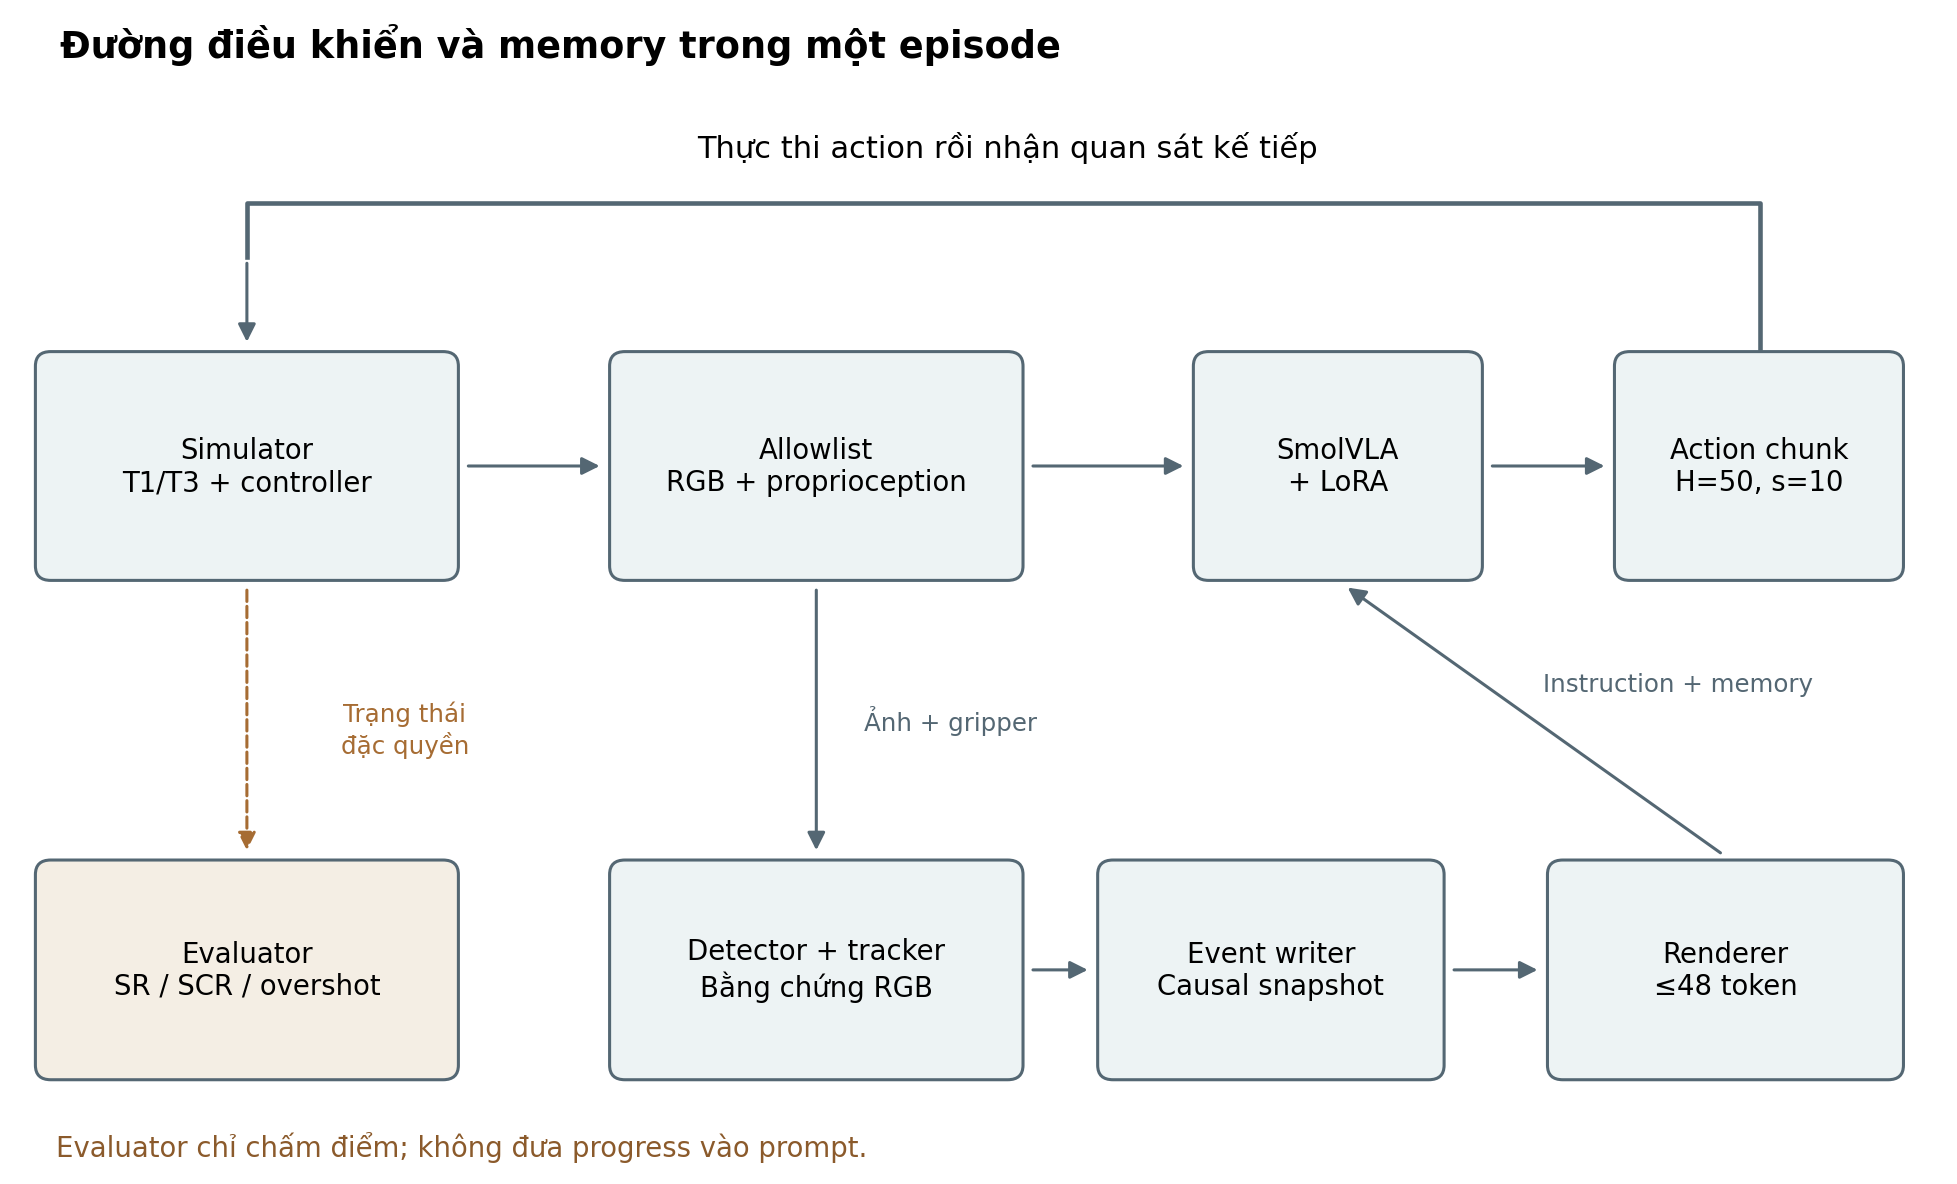
\includegraphics[width=\textwidth]{../figures/architecture.png}
\caption{Đường thông tin của phương pháp. Bộ nhớ được suy từ quan sát đã nhận, còn tiến độ do môi trường ghi nhận được dành cho đánh giá.}
\label{fig:architecture}
\end{figure}

Sự phân tách này đặc biệt quan trọng khi sinh mẫu huấn luyện từ quỹ đạo ghi sẵn. Một quỹ đạo đầy đủ có cả trạng thái sau thời điểm tạo mẫu và kết quả cuối lượt. Khi xây dựng ngữ cảnh cho một mẫu tại bước $t$, bộ ghi được cập nhật theo thứ tự thời gian và chỉ dựa trên tiền tố quan sát đến $t$. Thời điểm đủ bằng chứng cho từng sự kiện được lưu riêng để kiểm tra quy tắc này.

\section{Ước lượng quan hệ bát và đĩa gốc}

Giả định đo lường là trong bố trí của T1 và T3, một số thay đổi quan hệ bát và đĩa có thể được phát hiện từ chuyển động tương đối của các hộp giới hạn trong ảnh camera ngoài. Camera cổ tay cung cấp bằng chứng bổ trợ về khả năng quan sát. Đĩa gốc được neo bằng quan sát ở đầu lượt khi quan hệ bát trên đĩa đủ rõ và tay kẹp đã mở. Các quan sát sau phải ghép được với đĩa đã neo. Việc cố định tham chiếu theo thời gian giúp phép đo bám vào ngữ nghĩa “đặt về đĩa ban đầu”, kể cả khi bát xuất hiện gần đĩa khác.

Gọi $\mathbf b_t$ và $\mathbf q_t$ là tâm mép dưới hộp giới hạn của bát và đĩa ở bước $t$. Gọi $\mathbf b_0,\mathbf q_0$ là tọa độ tại lúc xác lập mốc tham chiếu, còn $w_b,h_b$ là chiều rộng và chiều cao hộp của bát tại thời điểm đó. Bộ theo dõi dùng ba đại lượng.

\begin{equation}
\begin{aligned}
d_t &= (\mathbf b_t-\mathbf q_t)-(\mathbf b_0-\mathbf q_0),\\
D_t &= \left\|d_t\oslash(w_b,h_b)\right\|_2,\qquad
L_t = -d_{t,y}/h_b .
\end{aligned}
\end{equation}

Ký hiệu $\oslash$ là phép chia theo từng thành phần. $D_t$ đo độ lệch khỏi quan hệ hình học lúc khởi đầu, đã chuẩn hóa theo kích thước biểu kiến của bát. $L_t$ đo thành phần dịch chuyển hướng lên trên mặt ảnh. Bộ theo dõi kết hợp $D_t$, $L_t$, tỷ lệ kích thước và độ ổn định theo thời gian. Độ mở đo từ hai khớp ngón kẹp bổ sung căn cứ cho việc xác nhận trạng thái nghỉ. Các ngưỡng trong cấu hình nghiên cứu được trình bày ở Bảng 3.1.

\begingroup\small\setlength{\tabcolsep}{4pt}\renewcommand{\arraystretch}{1.15}
\begin{longtable}{>{\raggedright\arraybackslash}p{\dimexpr 0.25\textwidth-2\tabcolsep\relax}>{\raggedright\arraybackslash}p{\dimexpr 0.35\textwidth-2\tabcolsep\relax}>{\raggedright\arraybackslash}p{\dimexpr 0.4\textwidth-2\tabcolsep\relax}}
\caption{Ngưỡng đo quan hệ giữa bát và đĩa gốc}\label{tab:generated2}\\
\toprule
\textbf{Đại lượng} & \textbf{Quy tắc trong cấu hình} & \textbf{Vai trò trong phép đo} \\
\midrule\endfirsthead
\toprule
\textbf{Đại lượng} & \textbf{Quy tắc trong cấu hình} & \textbf{Vai trò trong phép đo} \\
\midrule\endhead
\bottomrule\endfoot
Điểm phát hiện & $s_{\mathrm{det}}\ge 0{,}15$ & Lọc các hộp đề xuất theo điểm của bộ phát hiện \\
Tín hiệu nâng & $L_t\ge 0{,}40$ và nằm ngoài vùng gần đĩa gốc & Tạo ứng viên rời đĩa \\
Gần đĩa gốc & $D_t\le 0{,}30$. Tỷ lệ rộng từ $0{,}6$ đến $1{,}5$, cao từ $0{,}3$ đến $1{,}5$ & Tạo ứng viên quay về theo hình học ảnh \\
Ổn định & Độ dịch chuẩn hóa của tâm mép dưới $\le 0{,}15$ & Xác định bát ổn định so với quan sát gần nhất \\
Tay kẹp mở & Tổng trị tuyệt đối vị trí hai khớp ngón $\ge 0{,}055$ m & Bổ sung căn cứ để xác nhận bát đã được thả \\
Xác nhận theo thời gian & Ba quan sát phù hợp liên tiếp & Giảm xác nhận do nhiễu ở một khung ảnh \\
Ghép đĩa gốc & Độ dịch chuẩn hóa theo kích thước hộp đĩa neo $\le 0{,}45$ & Duy trì cùng đối tượng tham chiếu \\
Thu nhận mốc đĩa & Trong 20 bước đầu & Giới hạn thời điểm xác lập quan hệ ban đầu \\
\end{longtable}
\endgroup

Các phép đo trên mặt ảnh là chỉ dấu gián tiếp của quan hệ vật lý trong không gian ba chiều. Điểm phát hiện được dùng như tiêu chí chọn hộp, với ý nghĩa xác suất chưa được hiệu chuẩn. Trong trường hợp có nhiều hộp đề xuất, quan sát gần nhất có thể hỗ trợ ghép danh tính trong một khoảng thời gian giới hạn. Việc xác nhận ở bước hiện tại vẫn đòi hỏi quan sát phù hợp tại chính bước đó. Khi không định danh được bát hoặc không ghép được đĩa gốc, quan hệ ở bước hiện tại được ghi là chưa xác định. Các đặc điểm này giới hạn phạm vi áp dụng ở những cảnh có bố trí và góc nhìn tương tự.

\section{Ghi sự kiện và bất biến đếm chu kỳ}

Bộ ghi biểu diễn mỗi chu kỳ bằng một sự kiện rời đĩa và một sự kiện quay về theo đúng thứ tự. Quan hệ ban đầu được xác nhận khi bát ở gần đĩa gốc, ổn định và tay kẹp mở qua đủ số quan sát. Sau đó, tín hiệu nâng kéo dài tạo một sự kiện rời đĩa. Khi đã xác nhận sự kiện này, bộ ghi mới xét chuỗi quan sát bát về gần đĩa gốc, ổn định và tay kẹp mở để xác nhận sự kiện quay về. Mỗi lần xác nhận quay về kết thúc chu kỳ đang mở và tăng $\hat z_t$ một đơn vị.

Bộ ghi dùng trạng thái ứng viên để tích lũy bằng chứng. Khi bước quan sát bị bỏ qua hoặc không đủ căn cứ thị giác, ứng viên chưa xác nhận được xóa và cờ lịch sử chưa đầy đủ được đặt. Các sự kiện đã xác nhận được giữ. Nếu một chu kỳ đã mở trước khoảng trống, nó vẫn mở cho đến khi bộ ghi có bằng chứng phù hợp để xác nhận quay về. Số khoảng trống phản ánh mức độ gián đoạn của quan sát. Khi một khoảng trống có thể chứa sự kiện chưa được ghi nhận, từ $\hat z_t$ chưa thể khôi phục chính xác $z_t$. Nếu mọi lần quay về được xác nhận đều tương ứng đúng với các sự kiện thật phân biệt, $\hat z_t$ có thể được diễn giải như một cận dưới của số chu kỳ. Điều kiện đó cần được kiểm tra bằng dữ liệu có nhãn phù hợp.

\textbf{Mệnh đề 1 (bất biến đếm chu kỳ).} Trong một lượt thực thi với bộ ghi khởi tạo mới và các chuyển trạng thái hoàn tất theo quy tắc trên, mỗi lần tăng $\hat z_t$ đóng đúng một sự kiện rời đĩa đã xác nhận và chưa ghép cặp. Giữa hai lần tăng liên tiếp phải có một sự kiện rời đĩa mới.

\textbf{Chứng minh.} Gọi $J_t$ là số sự kiện rời đĩa đã xác nhận và $\chi_t\in\{0,1\}$ là cờ cho biết có một chu kỳ đang mở. Ở trạng thái khởi tạo, cả ba biến đều bằng không. Xét đẳng thức bất biến

\begin{equation}
J_t-\hat z_t=\chi_t.
\end{equation}

Chuyển xác nhận rời đĩa chỉ xảy ra khi $\chi_t=0$ trước chuyển và làm tăng $J_t$ một đơn vị đồng thời đặt $\chi_t=1$. Chuyển xác nhận quay về chỉ xảy ra khi $\chi_t=1$ trước chuyển và làm tăng $\hat z_t$ một đơn vị đồng thời đặt $\chi_t=0$. Các chuyển còn lại giữ nguyên $J_t$, $\hat z_t$ và $\chi_t$. Do đó đẳng thức đúng sau mọi chuyển theo quy nạp. Vì mỗi lần tăng $\hat z_t$ cần một chu kỳ đang mở và đóng chu kỳ đó, cùng một sự kiện rời đĩa chỉ ghép được với một lần tăng. Bất biến này ràng buộc cấu trúc của dãy sự kiện do bộ ghi tạo ra. Độ đúng của từng sự kiện so với thao tác vật lý còn phụ thuộc phép đo ở Mục 3.3.

\section{Tính không nhìn trước và biểu diễn văn bản}

Một sự kiện $e_j$ có thời điểm bắt đầu ước lượng $\tau_j$ và thời điểm đủ bằng chứng $\upsilon_j$. Chẳng hạn, nếu bộ ghi dùng ba khung ảnh liên tiếp từ bước 10 để xác nhận quay về, nó có thể gán $\tau_j=10$ và $\upsilon_j=12$. Sự kiện chỉ được sử dụng từ bước 12 trở đi. Tại bước truy vấn $q$, điều kiện thời gian và nguồn bằng chứng được biểu diễn bằng

\begin{equation}
\mathcal{E}_q =
\{e_j \mid \tau_j\le \upsilon_j\le q,\,
  \operatorname{source}(e_j)=\mathrm{RGB}\}.
\end{equation}

Nhãn nguồn $\mathrm{RGB}$ trong biểu thức chỉ các sự kiện do bộ theo dõi thị giác dự đoán và có căn cứ truy vết được. Bên cạnh thời điểm khả dụng, phép tạo văn bản kiểm tra sự nhất quán giữa danh tính bát, danh tính đĩa, số lần quay về và các sự kiện được tham chiếu. Dữ liệu lấy từ trạng thái đặc quyền của mô phỏng hoặc nhãn gán tay thuộc nguồn đánh giá. Phép tạo ngữ cảnh ở điều kiện F1 từ chối ảnh chụp bộ nhớ mang các nguồn này.

Chỉ dẫn gốc được giữ nguyên ở đầu ngữ cảnh. Phần bộ nhớ có thể mô tả số lần quay về đã xác nhận, chu kỳ đang mở hoặc lịch sử chưa đầy đủ. Ví dụ, ở bước truy vấn sau khi ghi nhận hai lần quay về trong T3, phần bổ sung có thể nêu rằng bát đã được quan sát quay lại đĩa gốc hai lần. Với lịch sử gián đoạn, cách diễn đạt phải thể hiện tính chưa đầy đủ của bằng chứng. Ngân sách là 48 token cho toàn bộ chỉ dẫn và phần bổ sung theo tokenizer của checkpoint, kể cả ký hiệu xuống dòng và token đặc biệt. Bộ dựng ngữ cảnh bỏ mệnh đề vượt ngân sách và ghi nhận lần bỏ đó. Chỉ dẫn tự vượt ngân sách làm dừng lượt chạy. Phạm vi của 48 token là đầu vào văn bản, còn số bằng chứng lưu trong suốt lượt có thể tăng theo độ dài quỹ đạo.

\textbf{Mệnh đề 2 (tính không nhìn trước của ngữ cảnh).} Cố định chỉ dẫn, cấu hình, định danh lượt và mọi nguồn ngẫu nhiên dùng để tạo bộ nhớ. Giả sử bộ ghi bắt đầu ở trạng thái mới, mỗi lần cập nhật chỉ nhận quan sát đến bước hiện tại và các hành động đã thực thi, đồng thời mỗi bằng chứng ảnh được ghép với đúng bước quan sát của nó. Giả sử phép tạo văn bản chỉ nhận trạng thái bộ nhớ hiện hành, kiểm tra $\upsilon_j\le q$ và từ chối các nguồn đặc quyền như trên. Khi đó, hai quỹ đạo có cùng tiền tố quan sát và hành động đã thực thi đến bước $q$ sẽ sinh cùng ngữ cảnh $c_q$, bất kể phần tiếp diễn của chúng.

\textbf{Chứng minh.} Cùng quan sát đầu và cùng cấu hình dẫn đến cùng trạng thái bộ nhớ ban đầu. Giả sử hai trạng thái bộ nhớ ở bước $t-1$ bằng nhau với $t\le q$. Hai tiền tố bằng nhau cho cùng $o_t$ và $a_{t-1}$, vì vậy quy tắc cập nhật $U$ cho cùng $m_t$. Quy nạp cho $m_q$ bằng nhau. Phép $R$ áp dụng cùng phép kiểm tra nguồn, thời điểm và ngân sách lên hai bản ghi giống nhau nên trả cùng $c_q$. Tính chất này có điều kiện trên việc cấp đúng bằng chứng quan sát theo thời gian. Nhãn nguồn và thời điểm được dùng để kiểm tra sự tuân thủ điều kiện đó. Độ đúng của nội dung sự kiện và mức độ chính sách sử dụng nội dung cần được xác định qua đánh giá thực nghiệm.

\section{Dữ liệu và thích ứng chính sách}

Dữ liệu thích ứng ghép các quỹ đạo mẫu LIBERO-10 với các quỹ đạo T1 và T3 từ bản phát hành của tác giả. Các quỹ đạo có cùng vector trạng thái khởi tạo được xếp vào cùng một nhóm trước khi chia tập. Định danh nhóm được tính từ vector đầy đủ ở biểu diễn float64 little-endian. Các nhóm từng dùng để phát triển bộ ghi được xếp vào tập huấn luyện. Cách chia này kiểm soát trường hợp cùng trạng thái khởi tạo xuất hiện dưới nhiều tên tác vụ hoặc mã quỹ đạo khác nhau. Lịch sử sử dụng tập kiểm tra trong phát triển và khả năng giao thoa với dữ liệu tiền huấn luyện vẫn ảnh hưởng đến diễn giải khả năng khái quát hóa.

Quy ước ảnh được xác định theo nguồn. Đối với hai camera, ảnh tinh chỉnh từ bản phát hành LIBERO-Mem được lật dọc một lần để trở về quy ước ảnh thô, còn ảnh kết xuất thô từ mô phỏng được giữ nguyên trước bộ tiền xử lý SmolVLA. Việc chuẩn hóa hướng ảnh giữ nguyên các phép biến đổi ảnh và quy tắc giải mã hành động của checkpoint. Adapter dùng trong Chương 4 được huấn luyện trên các quỹ đạo từ bản phát hành. Bộ dữ liệu phát lại theo cấu hình mô phỏng cục bộ còn cần hoàn tất kiểm chứng trước khi dùng để đánh giá một adapter mới.

Thích ứng được thực hiện bằng LoRA tại các phép chiếu query và value của attention trong mô-đun sinh hành động. Các trọng số nền được giữ cố định, cùng với bộ chuẩn hóa trạng thái và phép giải chuẩn hành động của checkpoint. Mỗi lô tối ưu hóa gồm dữ liệu thao tác cơ sở và dữ liệu T1/T3. Bộ lấy mẫu cân bằng theo tác vụ trong từng miền và chọn quỹ đạo trước khi lấy khung ảnh, nhằm hạn chế ảnh hưởng của chênh lệch độ dài giữa các quỹ đạo. Trộn dữ liệu cơ sở tạo điều kiện khảo sát khả năng duy trì kỹ năng sau thích ứng. Kết luận về khả năng duy trì đòi hỏi đánh giá chính adapter trên các tác vụ cơ sở dưới cùng quy trình.

\section{Thiết kế đối chứng}

Các đối chứng được xác định theo câu hỏi mà từng phép so sánh có thể trả lời. B0 là mốc tham chiếu với trọng số gốc. Để đo thay đổi do thích ứng, F0 cần dùng cùng tập quỹ đạo, cách chia, cấu hình, ngân sách huấn luyện và quy tắc chọn checkpoint như F1, với ngữ cảnh huấn luyện và suy luận chỉ chứa chỉ dẫn. F1 bổ sung biểu diễn sự kiện trong cả thích ứng lẫn suy luận. F1-off giữ nguyên trọng số F1 và bỏ phần sự kiện ở thời điểm suy luận.

\begingroup\small\setlength{\tabcolsep}{4pt}\renewcommand{\arraystretch}{1.15}
\begin{longtable}{>{\raggedright\arraybackslash}p{\dimexpr 0.29\textwidth-2\tabcolsep\relax}>{\raggedright\arraybackslash}p{\dimexpr 0.1775\textwidth-2\tabcolsep\relax}>{\raggedright\arraybackslash}p{\dimexpr 0.1775\textwidth-2\tabcolsep\relax}>{\raggedright\arraybackslash}p{\dimexpr 0.1775\textwidth-2\tabcolsep\relax}>{\raggedright\arraybackslash}p{\dimexpr 0.1775\textwidth-2\tabcolsep\relax}}
\caption{Các điều kiện đối chứng và mục đích đánh giá}\label{tab:generated3}\\
\toprule
\textbf{Điều kiện} & \textbf{Trọng số} & \textbf{Ngữ cảnh suy luận} & \textbf{Mục đích đánh giá} & \textbf{Bằng chứng hiện có} \\
\midrule\endfirsthead
\toprule
\textbf{Điều kiện} & \textbf{Trọng số} & \textbf{Ngữ cảnh suy luận} & \textbf{Mục đích đánh giá} & \textbf{Bằng chứng hiện có} \\
\midrule\endhead
\bottomrule\endfoot
B0 & Checkpoint gốc & Chỉ dẫn & Mốc tham chiếu trước thích ứng & 20 lượt T1/T3 \\
F0 & Adapter huấn luyện đối sánh & Chỉ dẫn & Đối chứng cho thay đổi do thích ứng & Chưa có lượt chạy đối sánh \\
F1 & Adapter học với bộ nhớ & Chỉ dẫn và sự kiện & Đánh giá phương pháp đề xuất & 20 lượt T1/T3 \\
F1-off & Cùng adapter F1 & Chỉ dẫn & Đo độ nhạy với việc bỏ phần sự kiện & Chưa có lượt chạy vòng kín \\
\end{longtable}
\endgroup

So sánh hiện có B0 với F1 đo chênh lệch khi thay đồng thời trọng số thích ứng và nguồn ngữ cảnh. So sánh F0 với F1 ở cùng ngân sách sẽ thu hẹp câu hỏi về giá trị của việc bổ sung nhánh bộ nhớ. Để nghiên cứu riêng giá trị của thông tin lịch sử, một đối chứng bổ sung có thể cung cấp tóm tắt quan sát hiện tại bằng cùng bộ phát hiện. Một đối chứng khác có thể giữ ngân sách token tương đương và dùng phần bổ sung không mang tín hiệu tiến độ. F1-off có ý nghĩa chẩn đoán độ nhạy của cùng trọng số với ngữ cảnh. Do phần bộ nhớ chưa được bỏ ngẫu nhiên khi huấn luyện F1, việc bỏ phần này lúc suy luận có thể đưa ngữ cảnh ra ngoài phân phối huấn luyện. Các đối chứng này xác định hướng kiểm tra giả thuyết mà các lượt B0 và F1 hiện có chưa phân giải được.

\section{Quy trình đánh giá và độ đo}

Hai cấu hình đã chạy dùng robot Panda với bộ điều khiển OSC\_POSE ở 20 Hz, hai ảnh kích thước $256\times256$ và cùng danh sách trạng thái khởi tạo đã khóa. Mỗi lượt có 20 bước làm nóng theo quy trình trước khi tính các bước của chính sách. SmolVLA dự đoán đoạn $H=50$ hành động và thực thi $s=10$ hành động trước khi truy vấn lại. Bộ ghi cập nhật sau từng hành động, vì sự kiện có thể được xác nhận giữa hai lần truy vấn.

Mỗi lượt có giới hạn 1.000 hành động do chính sách sinh và dừng sớm khi bộ chấm ghi nhận vượt mục tiêu. Một trạng thái hoàn tất xuất hiện giữa lượt vẫn phải được duy trì theo quy tắc chấm ở thời điểm kết thúc. Quy tắc này giữ yêu cầu kết thúc đúng tiến độ, vốn là phần quan trọng của tác vụ lặp. Bộ chấm đọc tiến độ và vị từ từ bản mã đánh giá LIBERO-Mem đã cố định phiên bản. Kết quả được diễn giải trong phạm vi quy trình mô phỏng cục bộ đã khai báo.

Với lượt $i$, gọi $K_i$ là số mốc được bộ chấm xác nhận, $K_i^\star$ là số mốc cần đạt, $P_i$ là vị từ đích tại thời điểm kết thúc và $O_i$ là cờ vượt mục tiêu. Gọi $M$ là số lượt hoàn tất đánh giá trong nhóm đang xét. Các độ đo gồm chỉ báo thành công $S_i$, tỷ lệ hoàn thành mốc $\mathrm{SCR}_i$ và tỷ lệ thành công thực nghiệm $\widehat{\mathrm{SR}}$.

\begin{equation}
\begin{aligned}
S_i &= \mathbf{1}[K_i=K_i^\star\land P_i\land\neg O_i],\\
\mathrm{SCR}_i &= K_i/K_i^\star,\qquad
\widehat{\mathrm{SR}} = \frac{1}{M}\sum_{i=1}^{M}S_i.
\end{aligned}
\end{equation}

$\mathrm{SCR}_i$ phản ánh tiến độ từng phần. $S_i$ còn yêu cầu trạng thái đích hợp lệ ở điểm cuối và dừng trong giới hạn số lần lặp. Hai tác vụ có cùng số lượt trong mỗi cấu hình đã chạy, nên trung bình tỷ lệ thành công theo tác vụ bằng tỷ lệ tính trên tất cả các lượt của cấu hình. Trạng thái khởi tạo được ghép giữa B0 và F1, đồng thời được dùng lại giữa T1 và T3. Cách ghép này cho phép đối chiếu từng trường hợp nhưng tạo phụ thuộc giữa các quan sát chung trạng thái. Việc phân tích vì vậy cần giữ thông tin nhóm trạng thái, số seed và điều kiện dừng của từng lượt.

